\chapter{Related Work}
\label{chapter2}
\thispagestyle{plain}

In the following sections we will describe methods and techniques related to the main pourpose of this work: automatically extract peaks using DEM data. In Section \ref{sec:mountain_peaks_from_dem} we will see more classical and heuristic methods of computer science which directly interact with DEMs for the identification of peaks. Section \ref{sec:deep_learning}, instead, is an introduction to \textit{Deep Learning}, the building block for the techniques used in the development of our workflow for learning how to extract peaks from graphs built over DEMs. 

\section{Mountain peaks extraction from DEM}\label{sec:mountain_peaks_from_dem}
One of the earliest attempts of extracting surface specific points, like peaks, from discrete terrain elevation data was done by K.Peucker and H.Douglas in  \cite{peackerAndDouglas}. They described several methods designed to detect landforms like pits, peaks, passes, ridges, ravines, and breaks, given an array of sampled, quantized terrain elevations. Their work analyzed topographic features of grid cells according to the patterns of elevation changes between neighbour cells.
The results are limited, as stated in \cite{lee1992modeling}, because of the encountered problems with single cell pits in flat areas due to high signal-to-noise
ratio.
Under the bigger landform detection problem goes the subproblem of moutains peaks identification. The pioneer work \cite{graff1993automated} introduces an automated method for classifying generic terrain features extracted from DEMs. Their two-class system differentiates mounts, the elevated features, and non-mounts, the remaining terrain features. Despite some limitations of the algorithm, also this work has been affected by the quality of digital data. Indeed, the authors of \cite{lee1992modeling} show how DEM errors affect the computation of the derived attributes. 
There exist six morphometric classes that can be identified in a DEM by analyzing the eight direct neighbours elevations, and an example can be seen in Figure \ref{fig:six_morphometric}.
\begin{figure} 
\centering
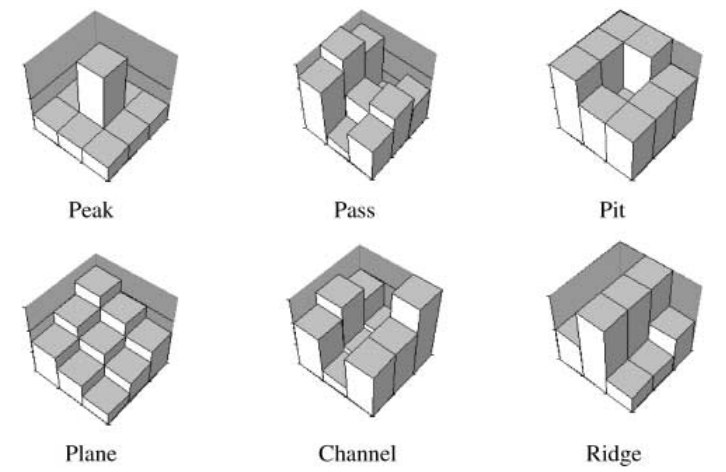
\includegraphics[width=12cm]{morphometric_classes.png}
\caption{Morphometric classes}
Figure illustrating the six morphometric classes that can be extracted from a raster DEM. Image courtesy Peter Fisher, Jo Wood and  T. Cheng \cite{fisher2004helvellyn}.
\label{fig:six_morphometric}
\end{figure}
Many studies and researches have been done to further extend the basic eight-neighbours method for extracting the morphometric classes. With a new perspective in \cite{fisherWhatIsAMountain} the authors show that based on the scale with which we analyze the terrains we can classify them differently. This goes in the direction of fuzzy set theory of terrain analysis. Peter Fisher, Jo Wood and  T. Cheng \cite{fisher2004helvellyn} explored the fuzziness of multi-scale landscape morphometry where they stated that any location can be allocated to a specific class, but the class to which a location is assigned may vary considering different scales. Indeed, an area that is a channel by considering its eight direct neighbours can be part of a ridge for a larger scale, considering, for example, not only the adjacent cells but also the ones that are connected to their neighbours. They showed how is it possible to combine classification at different scales for finding peaks.
The method is implemented in the Landserf\footnote{http://www.landserf.org/} application \cite{wood2009geomorphometry}. An example where we can see the fuzzy concept of "peakness", i. e. how much a given location belongs to the class of peak, can be seen in figure \ref{fig:landserf_app} (A) where red denotes a higher value of peakness. These techniques are further explored with a qualitative work in \cite{fisher2005fuzziness} and two use cases are reported: the Ben Nevis area, containing 19 peaks, and the Ainsdale coastal sand dunes. They show that some areas that have large value of peakness are actually corresponding to real peaks present in the dataset of known peaks used by authors, while some others are not associated with any summit.
\begin{figure} 
\centering
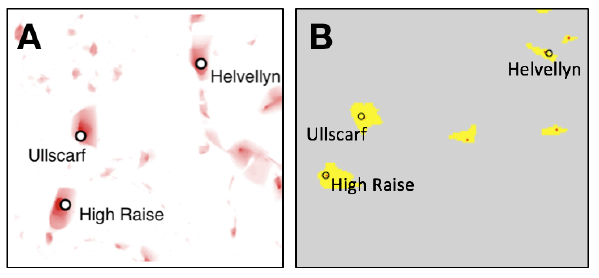
\includegraphics[width=14cm]{pictures/landserf_fuzzy_feature_extraction.png}
\caption{Landserf application}
(A) Landserf fuzzy feature extraction for peak classification and \\ (B) Landserf peak classification. Examples in a small area of Lake District using OS Terrain 50 DEM
\label{fig:landserf_app}
\end{figure}
The algorithm outcome is strongly influenced by its tunable parameters. The Landserf tool implements also a heuristic technique, based on the more classical method of the eight direct neighbours, which considers that a location may be considered a peak if its altitude is higher than a given treshold and there is a minimum elevation difference w.r.t its adjacent cells \cite{wood2009geomorphometry}. These quantities are two tunable parameters. An example can be seen in figure \ref{fig:landserf_app} (B). The yellow areas indicate the locations which are part of the extent of a mountain, while the red color denotes the summit of a mountains. With yet another approach, presented in \cite{schneiderWood}, and implemented in Landserf, the tool allows to extract peaks from DEMs also by building a so called \textit{Metric Surface Network}. It consists, essentially, in a graph with weighted edges whose vertexes are the critical points (peaks, pits and saddles) of a surface while the edges are the critical lines (channels and ridges). Also this method is subject to parameters tuning for optimization. Still considering 3x3 windows of DEM cells for the analysis of the locations for possible summits, the author of \cite{podobnikar2009method} and \cite{podobnikar2010mountains} combines topographic and morphologic criteria. According to these works a point, to be considered a peak, must reside in a non-flat area, must be the highest within its eight neighbors and must have at least a certain horizontal and vertical distance from other candidate peaks. The author, with a further qualitative study in \cite{podobnikar2012detecting} analyzes in detail the shape of a peak. By evaluating DEM data of the Kamnik Alps in Slovenia they show that shapes are dependent on each other and are not universal. The shape examination improves peak detection even though it is considered still as a very complex task to be generalized and solved by only authomated methods. 

Apart of studying the elevation of a cell relative to its adjacent ones, there have been developed also methods that considers the shape of a peak relative to its neighbours. Similarly to \cite{fisher2004helvellyn}, in \cite{deng2008multi} the authors consider mountains peaks as fuzzy entities and define a multi-scale peaks extraction algorithm based on local properties such as topographic position, number of summits in the neighborhood, relief, relative altitude and mean slope. The algorithm returns the peak class membership of a point expressed by a value suitable to further analysis through the application of a treshold. The effect of varying the treshold and the scale is presented through a qualitative evaluation. 

Other studies, like \cite{JASIEWICZ2013147} of J. Jasiewicz and F. Stepinski, focused in applying pattern recognition approaches for classifying and mapping landforms. They identified the so called \textit{geomorphon}, a simple ternary pattern that serves as base archetype for building more complex morphometric landforms. There are 498 geomorphons that constitute a comprehensive and exhaustive set of all possible morphological terrain types including all the standard elements of landscape, as well as unfamiliar forms. This approach of classification is significantly different from classical methodologies, indeed, it uses tools of computer vision rather than tools of differential geometry. The geomorphons can be then mapped to the more classical morphometrical classes. 

SAGA GIS \footnote{http://www.saga-gis.org/en/index.html} constitue another important tool in the field of landform detection. It has been usen in \cite{schillaci2} where the authors propose a worklow for Digital Terrain Analysis (DTA) and landform reconition and extraction from DEM. They analyze the most used terrain attributes, like slope, curvature and elevation, and combine different landfrom recognition methods, like digital topography. hidrology and morphology. The results show that different landforms are better characterized by different resolutions. In particular, higher resolutions allow to distinguish between more classes in the context of Fuzzy Landform Classification.

An important work based on heuristic approaches introduced in \cite{kirmse2017calculating} determines the \textit{prominence} and \textit{isolation} for the mountains, two important features characterizing peaks. Prominence is a measure of the independence of a summit and it is computed by finding the minimum vertical distance needed to descend from the peak to  to ascend to a higher one. Isolation, instead, measures the minimum distance of a summit from another one with higher elevation. For each peak in the world these two values are calculated and the results compared with the PeakBagger dataset \footnote{http://www.peakbagger.com/}. When computing the prominence for the summits a so called divide tree is built which represent the connection with the higher ones (except of the root of the tree which is the highest). These connections follow the path of descent from the peak until the lowest points, which is a saddle, before restarting to climb up a higher one. This tree can be thought like a sampling of the critical points and critical lines from the (metric) surface networks.


\section{Deep Learning}\label{sec:deep_learning}
Artificial Intelligence (AI) is the field that studies the creation of computer systems able to mimic the human cognitive functions in order to solve non trivial problems.
Machine Learning (ML) is a subfield of Artificial Intelligence that develops solutions that do not rely on explicitly programmed instructions to perform a certain task, but exploit a data-driven approach, in which patterns are learned from training data.
Learning can be supervised, semi-supervised or unsupervised \cite{DBLP:journals/corr/Schmidhuber14}. 
Furthermore, Deep Learning (DL) is a class of Machine Learning algorithms that relies on deep neural networks to learn data representations, which recently experienced great success,   thanks to the vast amount of training data and to the increasing computational power available nowadays.
DL models, have proved capable of achieving  high quality results in a wide range of Computer Vision tasks, such as image classification, detection, localization and segmentation.
In particular, it is easy to feed the above mentioned techniques, with euclidean data such as feature vectors, or images. The performance of Machine Learning algorithms heavily depend on the data they are fed with; the choice of the representation for the data on which they are applied requires important efforts on the design of preprocessing pipelines and data transformation. In cases were we have too much data engineering the relevant features  or when we’re in the domain of non-Euclidean data, the task of preparing the input to feed ML or DL models could be more challenging. To cope with this, there is a field called Rresentation Learning which goes in the direction of learning representations of the data that make it easier to extract useful information when building classifiers or other predictors. 
Deep Learning techniques are formed by the composition of multiple non-linear transformations with the goal of yielding more useful representations, as stated in \cite{DBLP:journals/corr/Schmidhuber14}.
The organization of the AI fields can be seen in Figure \ref{fig:AI_ML_DL}.
\begin{figure} 
\centering
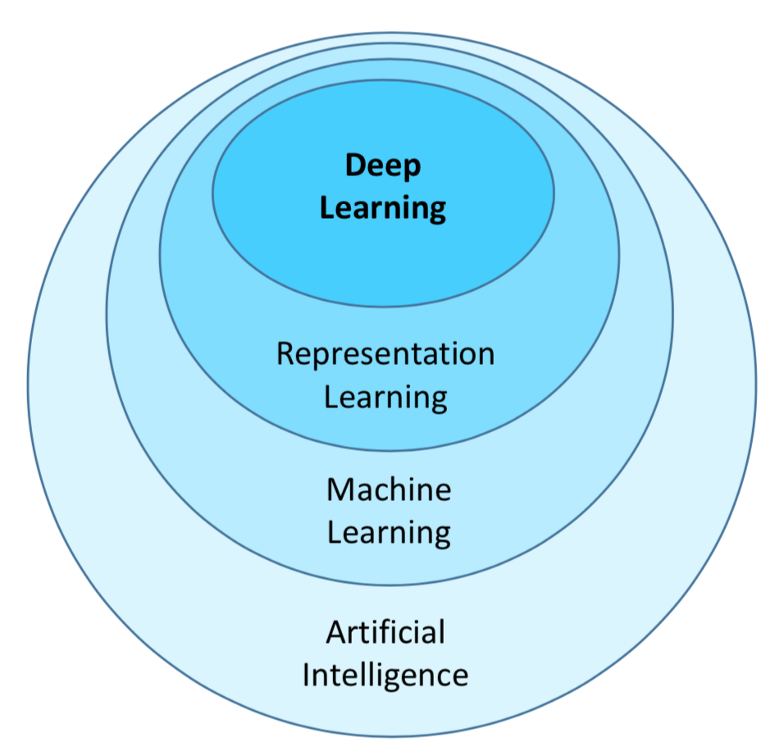
\includegraphics[width=10cm]{AI_ML_DL.png}
\caption{Artificial Intelligence fields}
Figure showing how Artificial Intelligence can be hierarchically organized in subfields. Deep Learning can be seen as a specific field of Representation Learning, that is by itself a specific field of Machine Learning, a subset of the broader class of Artificial Intelligence methods.
\label{fig:AI_ML_DL}
\end{figure}
In this section, we will do an overview of main concepts on these areas.

\subsection{Artificial Neural Networks}
The basic model over which are built many and more complex Deep Learning models are the so called Artificial Neural Networks, which are vaguely inspired by the biological neural networks that constitute animal brains. The neural network itself is not an algorithm but rather a framework for many different machine learning and, consequently, deep learning algorithms to work together and process complex data inputs. Their ability of learning from examples without being programmed for a specific task made them a breakthrough in many fields. Learning can be seen as as the process of adjusting internal parts of the model in order to approximate some unknown function \(f^*\), just by feeding the network with different examples of data. For example, for a classifier, \(f^*\) may be a function that maps an input \textbf{x} into a category \(y\). An artificial neural network defines a mapping \(\textbf{y} = f(\textbf{x};\boldsymbol{\theta}) \) where the values of the parameters $\boldsymbol{\theta}$ are learned such that \(f^*\) would result as the best approximation function. 

Artificial Neural Networks are based on a collection of connected units or nodes called artificial neurons whose connections, that have a shallow similarity with the biological synapses, can transmit a signal from one artificial neuron to another. Once a neuron receives a signal (usually represented by a real number) can process it and then send the outcome to the other neurons to which is connected. Generally, the output of each artificial neuron is computed by some non-linear function of the sum of its inputs, while the connections between artificial neurons are called edges. To the edges between neurons are then associated some weights that represent the strength of the connection and are the parts of the model that can be adjusted during the learning process. As we can see in Figure \ref{fig:neuron}, each  neuron \(i\) is fed with a vector of real numbers \(\textbf{x}\), i.e., the outcomes of the processing of the other neurons connected to \(i\); in this case we refer to \(x_j\) as the output of node \(j\) feeding node \(i\). Each input will be then multiplied by the weights $w_{ij}$ associated to the edges that connect the neurons \(j\) to neuron \(i\) and summed with the results of the other multiplications. There is, essentially, a dot product between the vectors \(\textbf{x}\) and \(\textbf{w}\) representing, correspondingly, the input data and the weights of the edges connecting the neurons. Then, the summation of the multiplications is used as an input to a non-linear activation function \(g\) which will produce the final signal \(y_i\). 

As an example of non-linear activation function we may consider the binary step (which is also present in Figure \ref{fig:neuron}) and write the output signal \(y_i\) as: 
\begin{equation}
  y_i = g(\textbf{x}) =
    \begin{cases}
      1 
      & \text{if } \textbf{x}
      \cdot
      \textbf{w}
       \: \geq 0 \\
      0 
      & \text{otherwise}
    \end{cases}
\end{equation}

\begin{figure}[htp] 
\centering
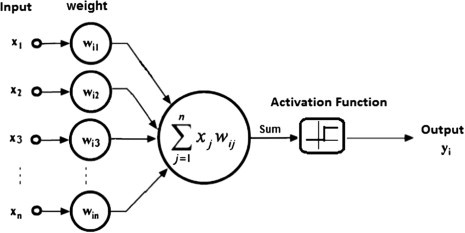
\includegraphics[width=12cm]{neuron.jpeg}
\caption{Artificial Neuron}
Figure taken from \cite{neuron} depicting the computational structure and the flow of information between neurons in an Artificial Neural Network.
\label{fig:neuron}
\end{figure}

One of the most well known example of ANN are the Feedforward Neural Networks, also called Multilayer Perceptrons (MLPs). As stated in \cite{Goodfellow-et-al-2016}, these models are called feedforward because information flows from \textbf{x}, which generally represents the data, through the intermediate computations used to define \(f\), and finally to the output \(\textbf{y}\). MLPs are acyclic, i.e they do not include feedback connections.

Feedforward Neural Networks are called networks because they are typically represented by composing together many different functions. An example may be $f(\textbf{x}) = f^{(3)}
(f^{(2)}(f^{(1)}(\textbf{x}))) $ where there are three functions $(f^{(1)}$, $f^{(2)}$ and  $f^{(3)}$ connected in a chain. Usually we say that the functions constitute the layers and we refer to $f^{(1)}$ as the first layer, $f^{(2)}$ as the second layer and so on. 

In Figure \ref{fig:deep_nn} we can see a general architecture of a (Deep) FNN. The difference between FNN and the deep ones consist in the number of layers. Deep FNN are in general composed by many more layers than the normal ones. It is important to highlight that the functions that constitute the chain can be cosidered as computational layers composed by different numbers of neurons. Essentially the stacked layers of neurons can be associated to the chain of funcions, and each layer's functionality is given by the combination of the processing units, i.e. the neurons, that constitute the layer. The layers can be then organized as: \(input \: layers\) (\(L_1\)), where the network is fed with the examples (usually constituted by vectors of real numbers), \(hidden \: layers\) (\(L_2, \: L_3, \: L_4\)), which usually receive the outcome of the computations of the input layers, and the \(output \: layers\) (\(L_5\)) that are fed with the signals coming from the hidden layers and whose output constitute the model response to the data. For example, if the model is trying to classify images, each different \(y_i\) representing the output may indicate the probability for the input picture to belong to a given class (cat, person, building, car, etc...). Organizing the neurons in layers allows to have powerful models that are able to learn really complex functions, or at least quite close approximations to an ideal \(f^*\). Also notice that this particular kind of Deep Feedforward Neural Network is a Fully-Connected one. As we can still see from Figure \ref{fig:deep_nn}, except of the input and output layers, each neuron from each layer is connected to all the neurons from the previous layer and to all the neurons of the next layer. The exception of the input and output layer is given by the fact that, as we said, the input layer receives the example so its neurons have no incoming edges from other neurons, while the output layer receives only the signals from the computations from the previous layer but is not feeding other layers since its result constitute the final approximation of the function \(f^*\).
The overall length of the chain gives the depth of the model, the term from which arose "deep learning"  name. 

\begin{figure}
\centering
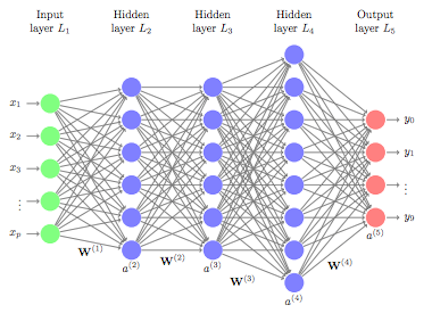
\includegraphics[width=12cm]{deep_nn.png}
\caption{A Deep Feedforward Neural Network}
Figure taken from \cite{deep_nn} showing the computational structure of a Deep (Fully-Connected) Feedforward Neural Network and the Layers that can be distinguished between input layers \(L_1\), hidden layers \(L_2\), \(L_3\),\(L_4\) and output layers \(L_5\). 
\label{fig:deep_nn}
\end{figure}

\subsection{The learning process}

As we said, the parts of the neural networks models which are usually modified to better approximate the objective function \(f^*\) are the edges connecting the neurons and their associated weights. Again as an example consider a supervised learning where human labeled data is used for training an artificial neural network that is classifying the content of images. The learning process is mainly constituted by three phases, the \textit{forward propagation}, the \textit{loss computation} and the \textit{backward propagation} (often named just \textit{backpropagation}). The first one occurs by feeding the network with examples, passing them across all the network and applying the transformations of each neuron. The outcome of the output layers can be interpreted as the network's prediction for the content of the image. After the output is calculated for each example that is given to the model, an error, usually called loss, is computed between what is the real content of the image and what is the neural network predicting. Here the last phase, the backpropagation, takes part. The loss is then propagated through all the neurons of the hidden layers and it is used to adjust the weights of the edges to reduce to the minimum the error. This process can be visualised in Figure  \ref{fig:backward_forward_propagation}.
\begin{figure}
\centering
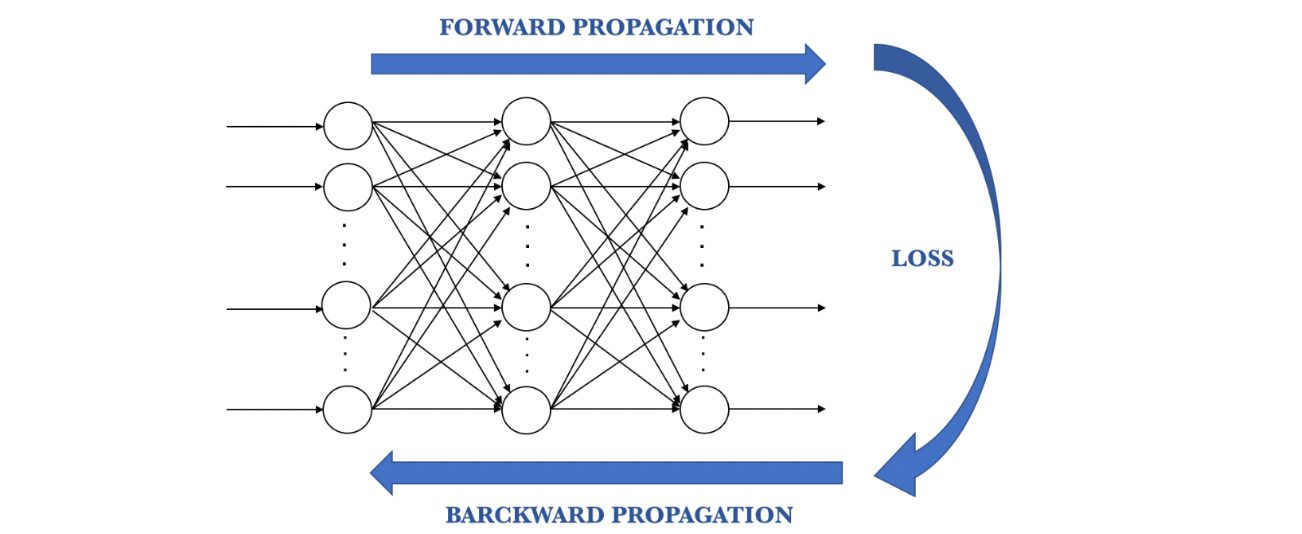
\includegraphics[width=15cm]{pictures/forward_backward_propagation.png}
\caption{Learning phases of a Neural Network}
Figure representing the learning phases of an Artificial Neural Network. (1) Forward propagation: the training data is passed across all the neural network and the outcome of the output layers represents the network's prediction. (2) Loss: represents how far the prediction is from the objective \(f^*\). (3) Backpropagation: the propagation of the loss to all the neurons in the hidden layers that contribute to the output. Image courtesy Jordi Torres \cite{backward_forward_propagation}
\label{fig:backward_forward_propagation}
\end{figure}
The objective is to make the loss as close as possible to zero the next time we will use the network for a prediction. For doing so, the \textit{gradient descent} technique it is used; it changes the weights of the edges with small increments by calculating the derivative (or gradient) of the loss function. Gradient descent tunes the weights in order to descend towards a \textit{global minimum} of the loss function of what is predicted against which are the real values of the examples. If we think at the neural network as a composition of functions, gradient descent tries to find the best \(\boldsymbol{\theta}^*\) for the function \(f(\textbf{x};\boldsymbol{\theta}) \) representing the network in order to minimize the loss between the ideal \(f^*\) and the actual approximating function \(f(\textbf{x};\boldsymbol{\theta})\).

\subsection{Deep Learning on GIS}
The latest improvements of Artificial Intelligence and Deep Learning made them suitable for replacing specific task algorithms. Also in the field of Computer Vision, for tasks such as image classification, detection, localization and segmentations \cite{guo2016deep}, the advancements of Deep Learning allowed a remarkable improvement of the performances compared to traditional methods. 
Specific models of Deep Learning, the Convolutional Neural Networks (CNN), have proved a great ability in dealing with images. As stated in \cite{long2015fully} they have been used in several works of geoscience and remote sensing as an important tool for the analysis of aerial images. Specifically, in \cite{audebert2016semantic} and \cite{marmanis2016semantic}, CNNs have been applied for aerial images segmentation, tackling land cover and objects mappings, in which each pixel is assigned a given class (e.g. road, car, vegetation, building, etc). Artificial Intelligence has been proved also of being effective for the analysis of DEM data. Models such as the Multilayer Perceptron have been applied in \cite{marmanis2015deep} for classifying the above-ground objects by having as main target the separation of the high-standing structures (trees and building) from their surrounding terrain.
In \cite{chen2016convolutional} the authors used DL on Airbone laser scanning (ALS) point cloud data for extracting digital terrain models (DTMs). Their method allows to classify points by using an image-like classification approach. Indeed, they map the relative height difference of each point with respect to its neighbours (in a square window) to an image. 

Digital Elevation Models in some areas of the Earth lack of good resolution. To overcome this problem in \cite{chen2016convolutional} the authors proposed the so called DEM super resolution, a technique that improves the resolution for a DEM on basis of some learning examples. With a different approach in \cite{guerin2017interactive} and \cite{beckham2017step} there have been suggested techniques which involve the synthetic generation of terrain images by using a specific model of DL, the Deep Generative Adversarial Neural Networks (GANs). 

Recently, the authors in \cite{AI3D-DL-PE} proposed the usage of CNN for extracting peaks from DEMs by creating patches of dimension 31x31x3 representing parts of the physical region delimited by the DEM. Each patch is a square of 31x31 pixels, where every pixel is a cell of the DEM raster containing the elevations. The patches containing the elevations are then treated like images, which makes them really suitable for models like CNN. The authors showed how is it possible to use Deep Learning methods to train a model with terrain data represented as DEMs capable of identifying mountain summits. Based on their work, we are extending the application DL for extracting peaks from digital elevation models by building graphs, specifically surface networks, over the DEMs and then applying Deep Learning on the graphs.

\subsection{Deep Learning on Graphs} \label{deep_learning_on_graphs}
In mathematics, and more specifically in graph theory, a graph is a structure amounting to a set of objects in which some pairs of the objects are in some sense "related". The objects correspond to mathematical abstractions called vertices (also called nodes or points) and each of the related pairs of vertices is called an edge (also called an arc or line) \cite{trudeau1993introduction}. Typically, a graph is depicted in diagrammatic form as a set of dots for the vertices, joined by lines or curves for the edges. An example of diagrams can be seen in Figure \ref{fig:graph}. 
\begin{figure}

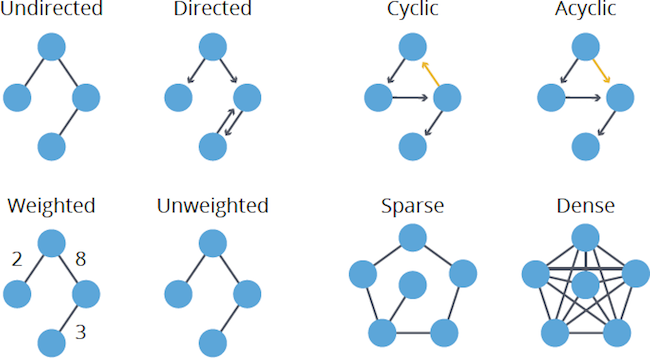
\includegraphics[width=13cm]{graph-properties.png}
\caption{Diagrammatic representation of the types of graphs}
The blue circles represent the vertexes (or the nodes), while the gray lines represent the connections among the nodes, i. e. the edges. The figure shows how can be defined 8 categories of graphs based on the type of edges.
\label{fig:graph}
\end{figure}

Graphs naturally exist in a wide diversity of real world scenarios, e.g., social graph in social media networks, citation graph in research areas, user interest graph in electronic commerce area, knowledge graph, etc. In Figure \ref{fig:graph} we can see a categorization of graphs based on their type of edges. For an \textit{undirected} graph, an unordered pair of nodes that specify a line joining these two nodes are said to form an edge. For a \textit{directed} graph, the edge is an ordered pair of nodes. If an edge is representing a relation in a family, for example a member \textit{father} of another member, the nodes represent the members while the directed edge represents in which direction is going the relation. In the context of directed graphs there can be made a distinction between \textit{cyclic} and \textit{acyclic} graphs, i.e if the graphs do contain a cycle or not. A cycle of a graph G is a subset of the edge set of G that forms a path such that the first node of the path corresponds to the last. A \textit{weighted} graph is a graph in which a number (the weight) is assigned to each edge. Such weights might represent for example costs, lengths or capacities, depending on the problem at hand. The \textit{unweighted} graphs, instead, do not have a cost associated or they all have the same cost usually set to 1. Also it can be distinguished between sparse or dense graphs. In the last ones there is an edge between all the possible pairs of vertexes in the graph, while in the sparse this is not happening.

\begin{figure}
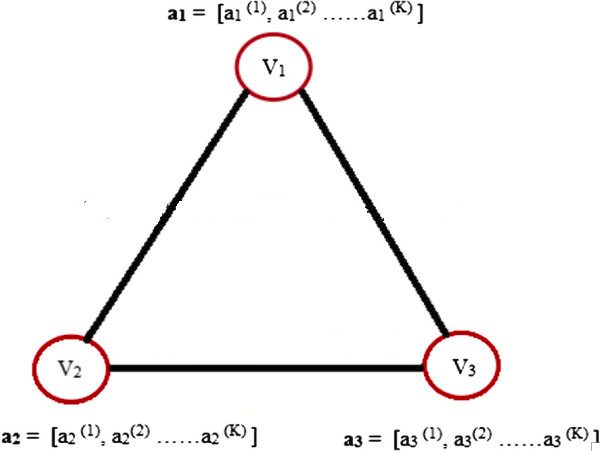
\includegraphics[width=8cm]{graph_with_features.png}
\centering
\caption{Graph with attributes}
The depicted graph is containing three vertexes and three edges. For each of the the nodes it is also present a vector \(a_i\) containing the properties of the node. In this particuar case each vector is composed by a fixed number K of attributes, arranged in an ordered list, from \(a_i^{(1)}\) to \(a_i^{(K)}\).
\label{fig:graph_with_attributes}
\end{figure}

There exist also graphs with features associated to the nodes, i.e. some numerical or categorical attribute representing properties in the domain of the graph. Figure \ref{fig:graph_with_attributes} shows a diagram representing such kind of graphs. 
For example if the graphs are representing sentences and the nodes are words, instances of attributes may be the length of the word, its position in the sentence and the word class (noun, verb, adjective, etc).

Being able to analyze properly these kind of graphs means being able to make good use of the information hidden in the structure of the graphs. An increased attention has been devoted to the topic in the last few decades \cite{surveyGraphEmbedding}. In particular, the utilization of Machine Learning on graphs became an important and ubiquitus task with applications ranging on very heterogeneous fields  \cite{representationLearning}. Examples of ambits of implementation go from classifying the role of a protein in a biological interaction graph, to predicting the role of a person in a collaboration network, from recommending new friends to a user in a social network to predicting new therapeutic applications of existing drug molecules whose structure can be represented as a graph. For achieving these tasks some typical problems need to be addressed on graphs. Usually node classification, link prediction and community detection are the main concerns, but also some other specific problem as a combination of the basic ones, such as subgraph classification or entire graph classification, can be evaluated. \textit{Node classification} aims to correctly classify the nodes as belonging or not to a given category. For example in a molecule the nodes may represent the atoms which we want to categorize as belonging to a chemical element. A diagrammatic representation of a molecule and its corresponding graph can be seen in Figure \ref{fig:molecule} (b). 
\begin{figure}
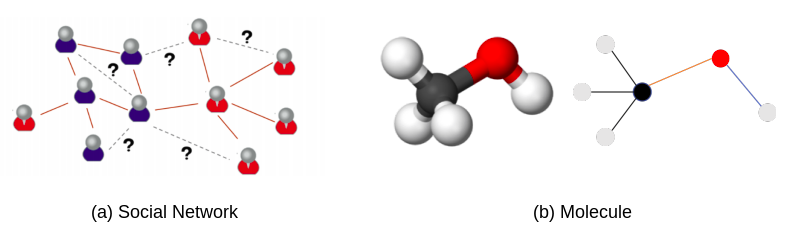
\includegraphics[width=14cm]{applications_graphs.png}
\centering
\caption{Graph models of reality}
Abstract representation two real world situations suitable for graphs. (a) Social Network instance with the members depicted as nodes and their relationships as edges. (b) Molecule representation where the nodes are the atoms and the edges are the molecular bonding. Image taken from \cite{graph_deep_learning}
\label{fig:molecule}
\end{figure}
\textit{Link prediction} problem, instead, goes in the direction of being able to predict the existence of a connection between two nodes and, more specifically, in the case of weighted graphs, the strength of the connection which can be represented by a real number. In Figure \ref{fig:molecule} (a) we can see an example where having a community of members represented with nodes we may want to predict a future connection, i.e. link prediction, among members which are not already in contact. \textit{Community detection}, instead, aims to cluster sets of nodes sharing specific properties that are intended to belong to a certain group. Figure 2.9 (a) can be an example where the two groups are formed by the members depicted in blue and red respectively. Other derived subproblems of the above described ones can be, for example, \textit{subgraph classification} where the purpose is to classify entire portions of the original graph, comprehensive both of the nodes and the edges. \textit{Graph classification}, instead, aims at classifying the entire graph with a category from a given domain. Still in the context of molecules, the purpose may be to classify the graph as "drug" or "non drug". Many machine learning applications seek to make predictions or discover new patterns using graph-structured data as feature information.

ML can automate functions, such as image classification, that are easy for a human to do, but hard to turn into a discrete algorithm for a computer. Deep learning allows us to transform large pools of example data into effective functions to automate that specific task. This is doubly true with graphs; they can differ in exponentially more ways than an image or vector thanks to the open-ended relationship structure. The central problem in machine learning on graphs is finding a way to incorporate information about the structure of the graph into the machine learning model. Graphs usually lack of a common structure either between two different graphs refering to the same domain, either among the nodes and the edges of the same graph. For example in a situation where two graphs represent two different communities, with the nodes representing the individuals and the edges representing the relations among the nodes, it would be really improbable to have the same number of nodes and edges. Also among the same graph the vertexes are generally having different numbers of edges connecting to their neighbours. Traditional methods that use machine learning algorithms with graphs rely on handcrafted features for encoding the graph structural information. Also, using directly the graphs as input for machine learning algorithms has a high computational and space cost \cite{surveyGraphEmbedding}. Recent approaches overcome the problem by learning \textit{graphs embeddings}, i.e. converting graphs into low dimensional space in which the graph information is preserved. This allows to use the embeddings of the graps as input to downstream machine learning models. Methods that create embeddings from graphs are part of the field of representation learning \cite{representationLearning}. There exist, however, also deep learning models which are able to handle directly graphs as inputs for performing tasks such as classification and regression of the entire graph, parts of it or its nodes. Standard machine learning algorithms generally rely on grid data structures (in 1, 2 and 3 dimensions). Convolutional Neural Networks (CNNs), one of the most successful examples of deep learning algorithms, exploit grid data structures and the translational equivalence/invariance with respect to this grid  \cite{spectral_networks_local_connected_networks}. One of the key challenges of extending CNNs to graphs is the lack of vector-space structure and shift-invariance making the classical notion of convolution elusive \cite{cayley_nets}. In their work, the authors of \cite{spectral_networks_local_connected_networks} showed how is it possible to extend these properties for graphs.
Then, even though the distincion is not sharp and the two categories may overlap, deep learning on graphs can be distinguished mostly in two groups of methods: representation learning through graph embedding and graph deep learning with direct application of the models over the graphs. 

\subsubsection{Graph Embedding}
As stated in \cite{surveyGraphEmbedding}, the problem of graph embedding is related to two traditional research problems: graph analytics and representation learning. Particularly, graph embedding aims to \textit{represent} a graph as \textit{low dimensional} vectors while the graph structures are preserved. Previous work addressed to this problem as a pre-processing step using hand-engineered statistics, such as node degree, to extract structural information. In contrast, representation learning approaches treat this problem as a machine learning task itself, using a data-driven approach to learn embeddings that encode graph structure \cite{representationLearning}.
In their survey the authors of \cite{surveyGraphEmbedding} show a graph embedding taxonomy based on the problem setting and on the used technique. This distinction is showed in Figure \ref{fig:taxonomy_graph_embedding}. 
\begin{figure}
\centering
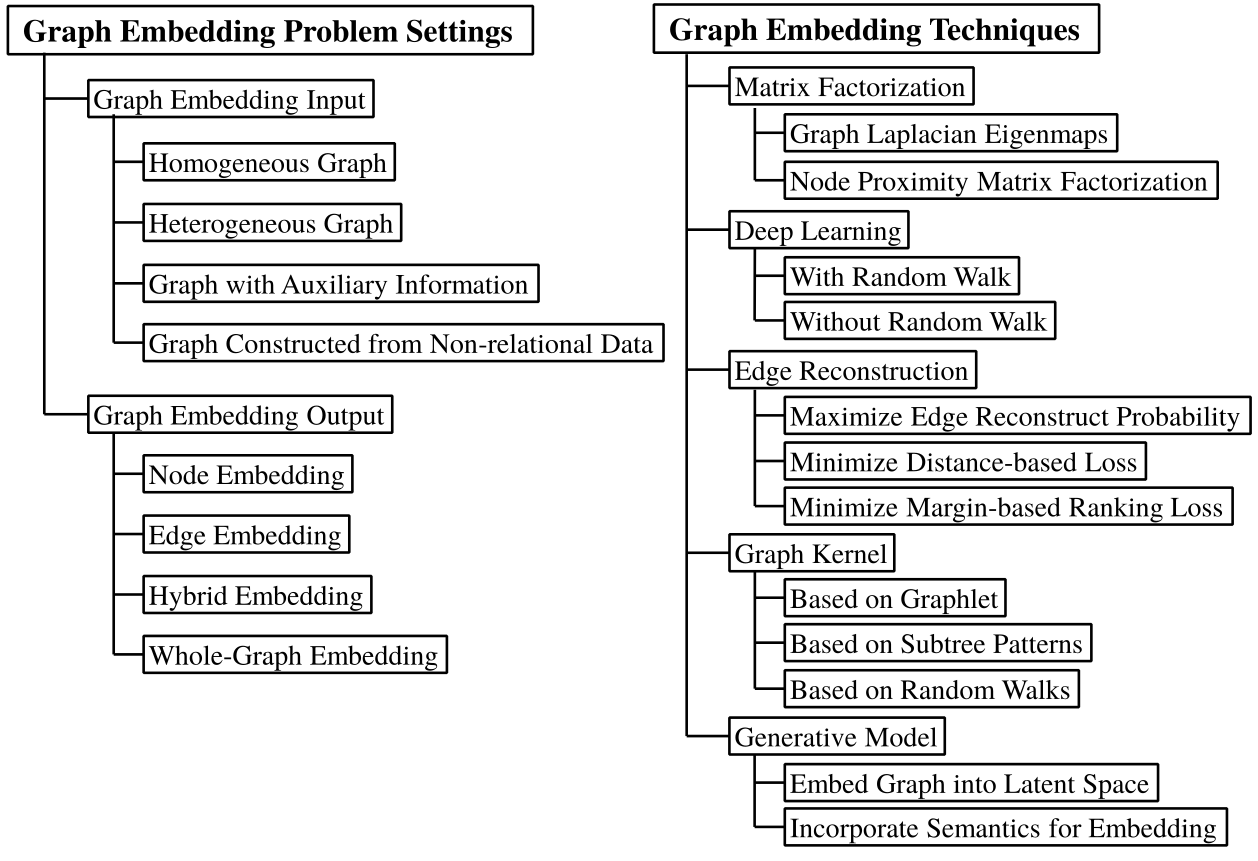
\includegraphics[width=14cm]{pictures/taxonomy.png}
\caption{Graph Embedding}
Figure taken from \cite{surveyGraphEmbedding} representing the taxonomy of graph embedding.
\label{fig:taxonomy_graph_embedding}
\end{figure}

Most of the embedding methods work in an \textit{unsupervised} manner, i.e. the algorithms have no prior knowledge about how the embeddings should be done or for which downstream machine learning task the embeddings will be used. There exist however also some graph embedding approaches which can be categorized as \textit{supervised} which make use of regression numerical attributes or classification labels in order to optimize the embeddings. 

In the context of unsupervised node embedding a really common \textit{framework} is the so called \textit{encode-decode} one where the \textit{encoder} maps each node to a low-dimensional vector (the embedding), while the \textit{decoder} decodes structural information about the graph from the learned embeddings (Figure \ref{fig:encoding_decoding}). 
\begin{figure}
\centering
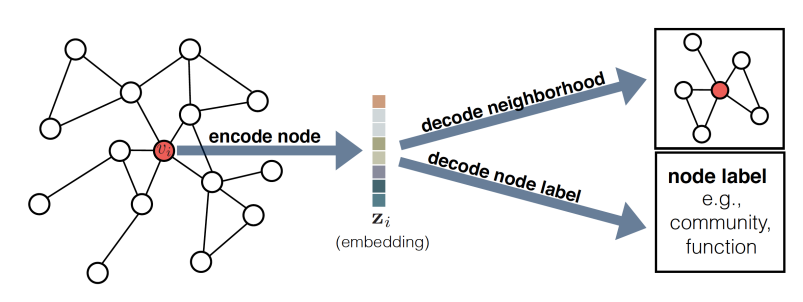
\includegraphics[width=14cm]{encoder-decoder.png}
\caption{Encoder-decoder approach}
Figure taken from \cite{representationLearning} representing an overview of the encoder-decoder approach. First, the encoder maps the node, \(v_i\), to a low-dimensional vector embedding, \(\textbf{z}_i\), based on the node's attributes and/or local neighborhood structure. Then, the decoder extracts user-specified information from the low-dimensional embedding, which can be the local neighborhood of \(v_i\) or a classification label associated to \(v_i\). By jointly optimizing the encoder and decoder the system learns to compress information about graph structure.
\label{fig:encoding_decoding}
\end{figure}
The vast majority of the works use a \textit{pairwise decoder} which assigns a graph proximity measure (expressed by real a value) to pairs of embeddings, i.e quantifies the proximity of the two nodes in the original graph. Applying such decoder to a pair of embeddings (\(\textbf{z}_i\),\(\textbf{z}_j\)) returns a \textit{reconstruction} of the proximity between \(v_i\) and \(v_j\) in the original graph. Finally, a loss function \(\ell\) measures how far the decoded proximity value is from the real proximity value. According to the measure loss \(\ell\) the encoder is then tuned in order to produce embeddings that would minimize the distance between the decoded proximities and the real ones. 

Under the encoder-decoder framework we can find numerous methods for embedding graphs; their differences vary based on their encoding function, decoding funcion, proximity measure and loss function. For example, DeepWalk \cite{deepWalk} and node2vec \cite{node2vec}, two really adopted algorithms in graph embedding literature, are using deep learning with random walks statistics. In graph theory, given a graph and a starting point, we select a neighbor of it at random, and move to this neighbor; then we select a neighbor of this point at random,
and move to it. The (random) sequence of points selected this way is a
random walk on the graph. Their key innovation is optimizing the node embeddings so that nodes have similar embedding if they tend to co-occur on short random walks over the graph. Instead of using a deterministic measure of graph proximity, the methods based on random walks use a flexible and stochastic measure of graph proximity, which has led to superior performance in a number of settings \cite{performanceRandomWalk}. Both methods, however, are failing to leverage node attributes during encoding which can be a hard limitation considering that node attributes can be higly informative with respect to the node's position and role in the graph. Also, these methods are inherently \textit{transductive} like said in \cite{transductive}, i.e. they can only generate embeddings for nodes that were present during the training phase, and they cannot generate embeddings for previously unseen nodes unless additional rounds of optimization are performed to optimize the embeddings. This is highly problematic for domains that require generalizing to new graphs after training.
Other methods, like Deep Neural Graph Representations (DNGR) \cite{DNGR} and Structural Deep Network Embeddings (SDNE) \cite{SDNE} implement encoders that do not use only the graph structure in order to compress the information about a node's local neighbor but they incorporate also the information about the node. These two methods also differ from the previous ones because they use a \textit{unary decoder} instead of a pairwise one. However, also these approaches are not using attribute informations about the nodes and they are strictly transductive and cannot generalize across graps. They are also really costly because the dimension of the autoencoder is fixed and equal to the number of vertexes inside the graph which can be really a huge problem for graphs with millions of nodes.
Similarly, some recent node embedding approaches designed encoders that rely on a node's local neighborhood, but not necessarily the entire graph. The idea is to generate embeddings for a node by \textit{aggregating} information from its local \textit{neighborhood}. The aggregation in this context relies on nodes features or attributes to generate embeddings. For example, a social network might have text data (e.g., profile information) or the nodes of a molecule, i.e. the atoms, can have features regarding their chemical properties. The neighborhood aggregation methods leverage this attribute information to inform their embeddings. In cases where attribute data is not given, these methods can use simple graph statistics as attributes such as node degrees. These methods
are often called \textit{convolutional} because they represent a node as a function of its surrounding neighborhood, in a manner similar to the receptive field of a center-surround convolutional kernel in computer vision \cite{kipf_semi_supervised}. During the encoding phase the neighborhood aggregation methods build up the representation in an iterative/recursive fashion. As showed in \cite{representationLearning} the procedure can be represented with an algorithm whose pseoudocode can be seen  in Figure \ref{fig:algorithm_1}.
\begin{figure}
\centering
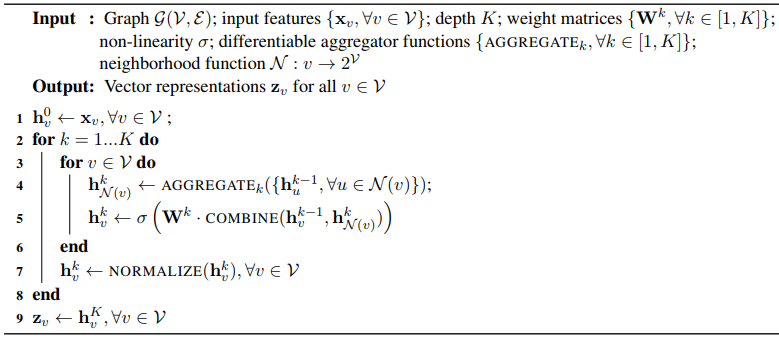
\includegraphics[width=14cm]{algorithm_1.png}
\caption{Neighborhood-aggregation encoder algorithm}
Figure taken from \cite{representationLearning} representing the pseudocode of the neighborhood-aggregation encoder algorithm.
\label{fig:algorithm_1}
\end{figure}
The initial node embeddings are set to be equal to the nodes attributes that are usually represented as vectors. At each iteration of the encoder algorithm, nodes aggregate the
embeddings of their neighbors, using an aggregation function that operates over sets of vectors. Then, for each node, the  aggregated neighborhood vector is combined with the node's previous embedding of the last iteration generating a new embedding which will be assigned to the node. Finally, this combined embedding is fed through a neural
network layer and the process repeats. As the process iterates, the node embeddings contain information aggregated
from further and further reaches of the graph. The encoder is forced to compress all the neighborhood information into a low dimensional vector such that, as the process iterates, the dimensionality of the embeddings remain constrained. After K iterations the process terminates and the final embedding vectors are output as the node representations. Different recent approaches fall into the setting illustrated in the algorithm of figure \ref{fig:algorithm_1}. Graph Graph Convolutional Networks (GCN) \cite{kipf_semi_supervised}, column networks \cite{column_networks} and GraphSAGE \cite{graphSAGE} all follow the neighborhood aggregation principle but differ primarly in how the \textit{aggregation} (line 4) and vector \textit{combination} (line 5) are performed. These algorithms exploit a set of trainable parameters, i. e. the aggregation functions and the weight matrices of the neural network layer \textbf{W}, which specify how to aggregate information from a node's local neighborhood. Differently from the encoder-decoder approaches listed before, the neighborhood aggregation encoder algorithm share the trainable parameters across the nodes. The parameter sharing increases efficiency (i.e. the parameter dimensions are independent of the size of the graph), provides regularization, and allows this approach to be used to generate embeddings for nodes that were not observed during training \cite{graphSAGE}. Also, differently from the algorithms of the encoder-decoder framework which are by default unsupervised, the neighborhood aggregation approaches can also incorporate task-specific supervision from node classification tasks in order to learn the embeddings. The task-specific supervision can be seen as a different way of computing the loss between the embedded vector and the desired one represented by the supervision. This allows for more fine tuned embeddings depending on the task we want to achieve. 

Based on the convolutional node embedding algorithms it is possible also to define subgraphs embeddings where the goal is to encode a set of nodes and edges into a low-dimensional vector embedding. The basic intuition behind these approaches is that they equate subgraphs with sets of node embeddings. They use the convolutional neighborhood aggregation idea (i.e., Algorithm in Figure \ref{fig:algorithm_1}) to generate embeddings for nodes and then use additional modules to aggregate sets of
node embeddings corresponding to subgraphs. An example is the work in \cite{molecular_fingerprints} where Duvenaud et al. introduced the so called “convolutional molecular fingerprints”, a \textit{sum-based} approach, where they create representations for subgraphs of molecular graphs by summing all the individual node embeddings in the subgraph. The node embeddings are generated using a variant of the Algorithm in Figure \ref{fig:algorithm_1}. Differently from the sum-based techniques where they sum the node embeddings for the whole graph, the \textit{graph-coarsening} approaches, such as the ones of Deferrard et al. \cite{deferrard} and Bruna et al. \cite{spectral_networks_local_connected_networks}, stack convolutional and "graph coarsening" layers. In the graph coarsening layers nodes are clustered together and the clustered node embeddings are combined using element-wise max-pooling. After clustering, the new coarser graph is again fed through a convolutional encoder and the process repeats. These approaches place considerable emphasis on designing convolutional encoders based upon the graph Fourier transform. Since naive versions of these encoders have complexity \(O(|V|^3)\), with |V| the number of vertexes, the authors of \cite{deferrard} introduce an approximation of the encoders by using the Chebyshev polynomials. However, as stated in \cite{representationLearning}, the introduced approximations make the graph coarsening methods conceptually similar to the algorithm in Figure \ref{fig:algorithm_1}.


Regarding the taxonomy showed in the survey \cite{surveyGraphEmbedding} for the graph embedding input in our work we focused on "graph with auxiliary information" with vector features representing properties of the nodes. For what concerns the output, instead, for our case was suitable to consider as objective the creation of "node embeddings" where for each node the embedding is a vector in a low dimensional space. We focused mainly on the "deep learning" embedding techniques because, as stated also in the survey, they are quite robust and effective and have been widely used in the field of graph embedding.


\subsubsection{Graph Deep Learning}
In Section \ref{deep_learning_on_graphs} we said that we wanted to distinguish between deep learning techniques aiming to create embeddings and the ones that learn directly on graphs. We refer as Graph Deep Learning techniques to the latter ones. However, this distinction is not sharp and the graph embedding techniques can be seen just as an intermediate step towards the global task of learning from graphs. Indeed,  the neighborhood aggregation approaches that can also incorporate task-specific supervision from node classification tasks can be seen as more general algorithms which apply directly deep learning over the graphs. They first learn how to encode the graph and then solve the specific ML task, such as classification, regression, etc., by applying more classical algorithms from ML literature. Indeed, we presented the GraphSAGE \cite{graphSAGE} model as a graph embedding technique which acts in an unsupervised manner. Nonetheless it can also be seen as a deep learning model that learns directly from graphs when incorporating supervised information such as labels for nodes. Also Deferrard et al. in their work \cite{deferrard} present their model not as an embedding algorithm but rather as a direct deep learning model on graphs which extends the concept of convolution from euclidean domains to irregular ones such as the graphs. The embedding step, however, as stated by \cite{representationLearning}, constitute an important part for these algorithms too, such that enables them to learn the proper representations for solving specific ML tasks. The models that rely on the Fourier transform, such as the one of Deferrard \cite{deferrard}, are called spectral models. As stated in \cite{monet} a key criticism of spectral approaches is the fact that the spectral definition of convolution is dependent on the Fourier basis (Laplacian eigenbasis), which, in turn is domain-dependent. It implies that a spectral CNN model learned on one graph cannot be trivially transferred to another graph with a different Fourier basis. In their work the authors of \cite{monet} solved partially the problem by being able to generalize over graphs with different number of edges. However, when dealing with tasks such as graph classification, their model still requires to keep fixed the number of nodes, i.e. the different graphs which are classified can have different number of edges but require to have the same number of nodes. Still in the context of spectral methods the authors of \cite{transfer_learning_on_graphs} attempted to advance deep learning for graph-structured data by incorporating another component: transfer learning. By transferring the intrinsic geometric information learned in the source domain, their approach can construct a model for a new but related task in the target domain without collecting new data and without training a new model from scratch.

In their work the authors of \cite{surveyGraphNeuralNetworks} proposed a categorization of the deep learning methods on graphs that can be seen in Figure \ref{fig:deep_learning_on_graphs}.
\begin{figure}
\centering
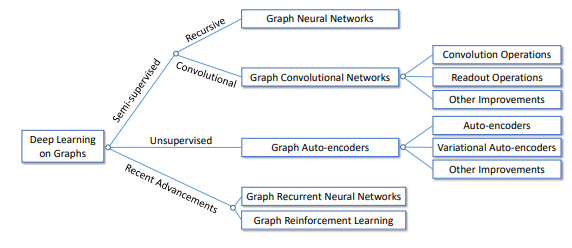
\includegraphics[width=14cm]{deep_learning_on_graphs.png}
\caption{Categorization of deep learning methods on graphs}
Figure taken from \cite{surveyGraphNeuralNetworks}. The authors divide the existing methods into three categories: semi-supervised, unsupervised
and recent advancements. The semi-supervised methods can be further divided into Graph Neural Networks and Graph Convolutional Networks based on their architectures. Recent advancements include Graph Recurrent Neural Networks and Graph Reinforcement Learning methods.
\label{fig:deep_learning_on_graphs}
\end{figure}
We worked mainly with the unsupervised deep learning methods,specifically with graph auto-encoders such as \textit{node2vec} \cite{node2vec}, and with the semi-supervised graph convolutional networks such as \textit{graphSAGE} \cite{graphSAGE} and the convolutional neural networks in the spectral domain of \cite{deferrard}. It is important to highlight that in our work the algorithms which are categorized as semi-supervised in \cite{surveyGraphNeuralNetworks} can be and have been used in a supervised context. In semi-supervised approaches only a few nodes have additional supervised inoformation such as node labels, i.e it is also used an amount of unlabeled data during training, while in the supervised cases all the nodes have such information. As we will see in Chapter \ref{chapter3} the graphs used in this work are the so called \textit{Surface Networks} where the nodes have attributes given by terrain conformation while the labels for the classification task is given by their category (peak / non peak).